% parte que saiu da tese
% Dados sobre a OSESP
% linguagem: LaTeX

\begin{comment}

\section{A Orquestra Sinfônica do Estado de São Paulo}



É senso comum entre os músicos e frequentadores das salas de concerto em São Paulo e ao longo do país que a OSESP é a principal orquestra brasileira. De fato, a OSESP é a orquestra com maior projeção internacional entre as brasileiras, com o maior orçamento, com a maior quantidade de discos gravados, etc. Além disso, foi a primeira orquestra brasileira que passou por um processo de reestruturação de seu modelo de gestão o qual foi também implementado em diversas outras instituições. Para \citeonline{arruda2010parcerias}, a experiência da OSESP é um grande êxito tanto em qualidade artística como na implementação eficiente de uma política cultural.



A OSESP foi criada em 1954 com a lei 2.733/1954 de São Paulo e teve o maestro Souza Lima como seu primeiro regente titular. Segundo \citeonline{marques2015osesp}



\begin{citacao}

Em 1997, a convite de Marcos Mendonça, então secretário de Estado da Cultura, John Neschling conduziu o processo de reestruturação, pautado pelas diretrizes formuladas por Eleazar [de Carvalho, o regente titular anterior]. Estas incluíam, além da nova sede, melhores salários para os músicos -- dos quais se esperava uma reavaliação mediante concurso interno. Dos 97 instrumentistas, 68 aceitaram fazer os testes e 44 foram aprovados, entre os quais os dois primeiros clarinetes, os oboés, uma primeira flauta, uma primeira trompa, os trompetes, os trombones, seis contrabaixos, a primeira viola, o \textit{spalla} e o naipe de percussão. Vinte e seis músicos foram contratados em Nova York, Paris, Bucareste e Sófia. A banca desses concursos internacionais era composta por Roberto Minczuk, maestro assistente da Osesp, e membros de orquestras como a Filarmônica de Viena e a Gewandhaus de Leipzig, além de solistas como o violoncelista Antonio Meneses e o violinista Régis Pasquier. \cite{marques2015osesp}

\end{citacao}



Além das melhorias descritas por \citeonline{marques2015osesp}, acreditava-se ser necessário entregar a gestão da OSESP e da Sala São Paulo, equipamento cultural de residência da orquestra, a uma entidade de direito privado visando maior eficiência, transparência e agilidade dos processos, já que, segundo \citeonline[p. 7-8]{arruda2010parcerias} ``a estrutura da administração pública, (\ldots), é completamente incompatível com as atividades e necessidades de uma orquestra sinfônica de categoria internacional, notadamente em razão de entraves burocráticos''. Essa transferência, a qual ocorreu de fato em 2005 com a criação da Fundação OSESP, foi embasada na Lei das Organizações Sociais do Estado de São Paulo -- Lei Complementar Estadual 846/98 -- que ``estabelece que entidades privadas portadoras de determinadas características, sem finalidade de lucro, poderão ser qualificadas, pelo Governador do Estado, como Organizações Sociais da Cultura ou da Saúde'' \cite[p. 6]{arruda2010parcerias}. Essa qualificação permite que essas OS's firmem com o estado um contrato de gestão, um termo jurídico no qual são estabelecidos direitos, deveres, controles, penalidades, metas, indicadores, etc., por meio do qual a gestão de uma atividade não exclusiva é delegada.



Em 2005, foi instituída a Fundação OSESP e firmado o primeiro contrato de gestão que vigorou até 2010.

Os objetivos da Fundação conforme seu estatuto são



\begin{citacao}

a. manter a ORQUESTRA SINFÔNICA DO ESTADO DE SÃO PAULO, assim como contribuir para a manutenção e melhoria do seu padrão de qualidade;\\

b. criar e manter Academia de Música, fomentando a educação e a cultura, especialmente no que tange à música;\\

c. realizar eventos e/ou ações educacionais para adultos, jovens ou crianças;\\

d. promover a educação, a capacitação e o treinamento de profissionais da área musical;\\

e. desenvolver programas de incentivo à formação de plateias para crianças e adultos;\\

f. desenvolver programas de acesso de alunos e docentes das escolas aos ensaios e concertos didáticos da Orquestra Sinfônica do Estado de São Paulo;\\

g. desenvolver e aperfeiçoar o Centro de Documentação Musical;\\

h. defender e conservar o patrimônio histórico e artístico e estimular e promover a promoção e a difusão de manifestações e bens culturais e artísticos de valor regional e/ou universal, formadores e informadores de conhecimento, cultura e memória, bem como que estimulem a liberdade de expressão;\\

i. fomentar a criação de espaços de expressão e criação artística e intelectual que contribuam para a promoção da cidadania, do acesso à música e às artes em geral;\\

j. difundir o repertório sinfônico e de câmara brasileiro;\\

k. desenvolver ações assistenciais que visem a integração ao mercado de trabalho e a inclusão social por meio da difusão e do ensino da música clássica e erudita;\\

l. incentivar a participação de regentes e solistas brasileiros com reconhecido mérito artístico;\\

m. oferecer bolsas e criar prêmios e/ou concursos e outras ações de estímulo relacionadas com seus campos de atuação;\\

n. difundir a música clássica, disponibilizando e/ou explorando apresentações para exibição por rádio e televisão, edição de obras de compositores brasileiros, gravação de CD's e DVD's e outras mídias, formação de plateias, aperfeiçoamento de instrumentistas, incentivo à colaboração voluntária e atividades afins;\\

o. estabelecer polo de gravação de música;\\

p. constituir Fundo de Capital ``\textit{endowment}'' e outros, caso necessário, para a Orquestra Sinfônica do Estado de São Paulo, a ser composto por doações, contribuições, recursos governamentais, eventuais excedentes financeiros e outros;\\

q. difundir e explorar marcas que possua ou detenha os direitos de exploração, quando para tanto autorizada;\\

r. apoiar ações e projetos da Orquestra Sinfônica do Estado de São Paulo, bem como desenvolver campanhas, realizar estudos e pesquisas, divulgar e distribuir informações, dados, trabalhos, documentos, entre outras atividades relacionadas com seus objetos;\\

s. apoiar a administração e o gerenciamento de espaços, inclusive negociar e receber por sua utilização por terceiros, quando para tanto autorizada, bem como prestar serviços relacionados aos seus objetivos, podendo também contratar a prestação de serviços de terceiros;\\

t. colaborar ou participar de programas governamentais ou desenvolvidos por entidades privadas ou da sociedade civil que afetem ou sejam afins às suas áreas de atuação, podendo, inclusive, participar e/ou aceitar assentos em Comitês, Câmaras, Fóruns, Redes e outros, assim como participar de outras pessoas jurídicas;\\

u. realizar quaisquer atividades ou praticar quaisquer atos necessários ou relacionados ao cumprimento de seu objetivo social.

\cite[p. 2]{osesp2013estatuto}

\end{citacao}



Para realizar seus objetivos, a Fundação detém certa autonomia para firmar contratos de gestão, parcerias, convênios, acordos com pessoas físicas, jurídicas, públicas ou privadas, nacionais ou internacionais.



O processo de negociação do contrato de gestão foi, para \citeonline{arruda2010parcerias}, bastante longo, complexo e intermitente tendo início em 2001. Para esse autor, o tempo de negociação, entretanto, foi necessário para aprendizado tanto dos gestores envolvidos quanto do poder público. Dois problemas apresentavam-se de maneira mais notória: o primeiro relacionado às questões jurídicas que envolvem um contrato de gestão. O instrumento era uma novidade para o Brasil naquela época e causava estranheza e resistência a alguns membros mais conservadores da administração pública. Além disso, não havia experiência em elaboração de contratos ou planos de trabalho e tampouco na escolha de metas e indicadores adequados. Para \citeonline[p. 9]{arruda2010parcerias} ``no caso das Organizações Sociais da Cultura, o aprendizado se deu na prática, de parte a parte, o que tornou a discussão mais lenta, mas não necessariamente menos produtiva e proveitosa''. Para esse autor a qualidade diferenciada dos trabalhos geridos pela Fundação bem como sua eficiência administravas advém desse longo período de maturação do contrato de gestão.



O terceiro desafio do novo modelo de gestão residia no orçamento. Havia tanto o problema da escolha dos destinos do investimento (investir na cultura era necessariamente investir menos em saúde ou educação, por exemplo) quanto a falta de uma contabilidade individualizada e detalhada. Segundo \citeonline{arruda2010parcerias}, isso acontecia porque



\begin{citacao}

dentro da administração pública as diversas `áreas' podem contribuir para a realização de um mesmo projeto e, ainda, devem adaptar suas atividades à flutuação do orçamento repassado a cada uma, ano a ano, flutuação essa que nem sempre está ligada a realidade da atividade, nem à demanda, mas sim a fatores externos, principalmente políticos e de arrecadação. \cite[p. 10]{arruda2010parcerias}

\end{citacao}



A Osesp, entretanto, parece ter empenhado esforços no sentido de manter uma contabilidade o mais racional possível desde o princípio apurando os custos envolvidos em toda a gama de atividades empreendidas (concertos, projetos educacionais, custos da Sala São Paulo, do Centro de Documentação Musical, etc.). Para firmar o contrato de gestão era necessário também estabelecer qual seria o impacto do novo modelo sobre os custos. Essa necessidade deu origem à elaboração de cenários que levavam em conta questões tributárias, societárias, trabalhistas e previdenciárias a parte dos quais o Governo adquiriu segurança para estabelecer valores corretos para a execução das atividades contratadas.



Após a fase de elaboração e revisão dos contratos de músicos e funcionários da OSESP, o próximo passo consistiu da elaboração de mecanismos de controle interno. Segundo \citeonline{arruda2010parcerias}, na orquestra não existiam departamentos de contabilidade e controladoria, recursos humanos, compras ou procedimentos administrativos padronizados. Boa parte desses serviços, no início, foram terceirizados até a implementação de um sistema integrado de gestão. O contrato de gestão, ao contrário do \textit{modus operandi} da administração pública o qual privilegia a lógica exclusiva da fiscalização formal do gasto, busca equilibrar a formalidade no gasto e o compromisso com os resultados nele implícitos. Por isso, é imprescindível que sejam constantemente aperfeiçoados as metas e os indicadores estabelecidos nele. ``As metas e os indicadores devem refletir com a maior precisão possível o que o Governo e o contratado esperam na execução da atividade'' \cite[p. 15]{arruda2010parcerias}. Alguns dos indicadores hoje utilizados são: número de concertos na Sala São Paulo, concertos gratuitos, concertos ao ar livre e fora de São Paulo (interior de SP, outros estados e exterior), porcentagem de ocupação dos eventos promovidos, número de concertos do Coro da OSESP, número de regentes e solistas convidados, número de concertos didáticos, gincanas musicais e professores treinados no programa educacional da instituição, número de cursos e oficinas promovidos, número de alunos da Academia da OSESP, número de concertos disponibilizados em TV e Rádio, horas de músicas disponibilizadas em podcasts, número de horas de obras gravadas, número de partituras editadas, número de encomendas de obras, número de obras estreadas, índice de satisfação do público com os concertos e com a Sala São Paulo, percentual de receitas próprias captadas pela Fundação OSESP, dentre outros \cite{osesp2014anexo1}.



A Fundação OSESP está submetida ao controle de diversas instituições do poder público (Secretaria de Estado da Cultura, Comissão de Avaliação das Organizações Sociais de Cultura, Secretaria de Estado da Fazenda, Tribunal de Contas, etc.) e da sociedade civil. Além disso, a Fundação tem uma controladoria interna que cuida do planejamento, gestão orçamentária e prestação de contas da instituição. Para \citeonline{arruda2010parcerias}



\begin{citacao}

A  necessidade  de  disponibilizar  as  informações  contábeis  e  financeiras, não  só  seu conteúdo,  mas  a  qualidade  e  o  tratamento dessas  informações, requerem que o gestor lance mão dos mais modernos recursos técnicos disponíveis, sendo que a construção de relatórios gerenciais e balancetes/balanços e orçamento, por  exemplo,  segmentados  por  origem  de recursos  (recursos  próprios,  contrato  de gestão, leis de incentivo), ou pela destinação (custeio, pessoal, compra de ativos) se tornam  desafiadores.  É  plausível  dizer  que  poucas  empresas  privadas,  mesmo algumas  do  setor  industrial,  vêem-se  na  obrigação  e necessidade de  controles  tão rígidos tais como as Organizações Sociais, pelo menos da forma como o Estado tem exigido até o momento. \cite[p. 16]{arruda2010parcerias}

\end{citacao}



Isso exige um certo nível de maturidade organizacional e familiaridade com os processos.



\subsection{Estrutura}



A Fundação OSESP é composta pelos seguintes órgãos:



\begin{enumerate}

\item[a] Conselho de Orientação;

\item[b] Conselho de Administração;

\item[c] Diretoria Executiva;

\item[d] Conselho Consultivo e

\item[e] Conselho Fiscal.

\end{enumerate}



O Conselho de Orientação é o órgão da instituição responsável pelas diretrizes estratégicas e institucionais para todos os outros órgãos. O Conselho de Administração é o órgão máximo de deliberação e orientação da instituição. Este órgão é o responsável pela promoção da política geral da instituição, pela designação e dispensa dos membros dos demais órgãos excetuando-se o Conselho de Orientação, indicação e dispensa de Diretor Artístico e Regente Titular da OSESP bem como decidir sobre o recebimento de doações e alienação de imóveis pertencentes à Fundação. A Diretoria Executiva é o órgão máximo de administração executiva da instituição e é composta por um Diretor Executivo e até dois Diretores Adjuntos. O Diretor Executivo é o responsável pela administração executiva geral da instituição. O Conselho Consultivo é um órgão de consulta e aconselhamento à disposição dos demais órgãos institucionais. Por fim, o Conselho Fiscal é o órgão de financeira e contábil da instituição \cite{osesp2013estatuto}. Essa estrutura com seus respectivos membros está representada na Figura 5.



\begin{sidewaysfigure}

\centering

\caption{A estrutura da Fundação OSESP 1}

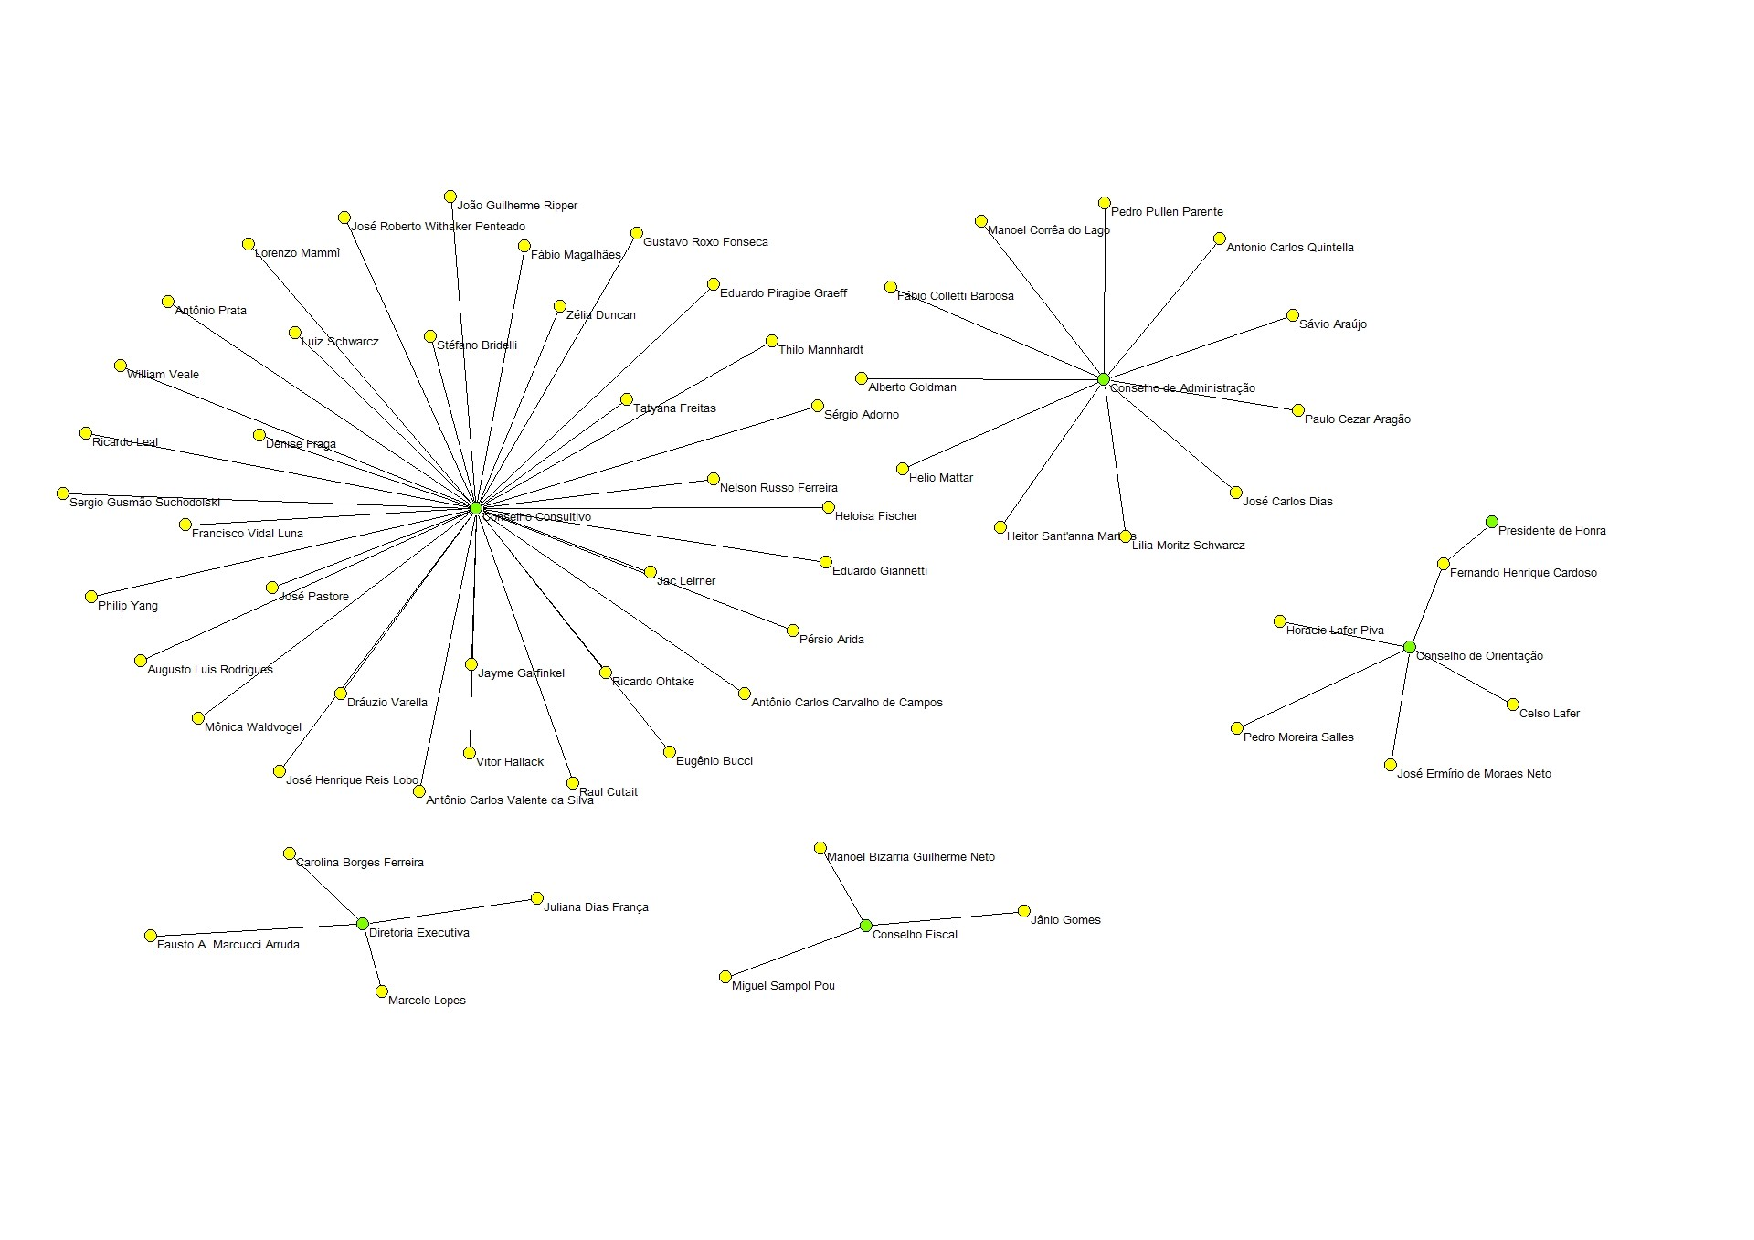
\includegraphics[scale=0.8]{OSESP_conselhos_pajek.pdf}

\fonte{Site da \citeonline{osesp2016site}. Dados trabalhados pelo autor.}

\end{sidewaysfigure}



Além dos órgãos supracitados, a Fundação OSESP contém em sua base setores artísticos, pedagógicos e administrativos. São eles a Diretoria Artística, a Orquestra, o Coro, a coordenação artístico-pedagógica do Festival de Inverno de Campos do Jordão (festival de cunho formativo mantido pela Fundação OSESP), departamento jurídico, o Centro de Documentação Musical e Editora Criadores do Brasil, o setor de Atividades Educacionais (responsável pela Academia da Osesp, máster-classes e demais projetos formativos), departamento de marketing, departamento de comunicação, controladoria, contabilidade, departamento financeiro, uma divisão administrativa (composta de gerência, recepção, serviços de copa, serviços terceirizados, recursos humanos, informática, almoxarifado e arquivo), e uma divisão operacional (composta de departamento de produção, departamento técnico, iluminação, som, montagem, departamento de operações, controlador de acesso e indicadores). Essa estrutura está representada na Figura 6.



\begin{sidewaysfigure}

\centering

\caption{A estrutura da Fundação OSESP 2}

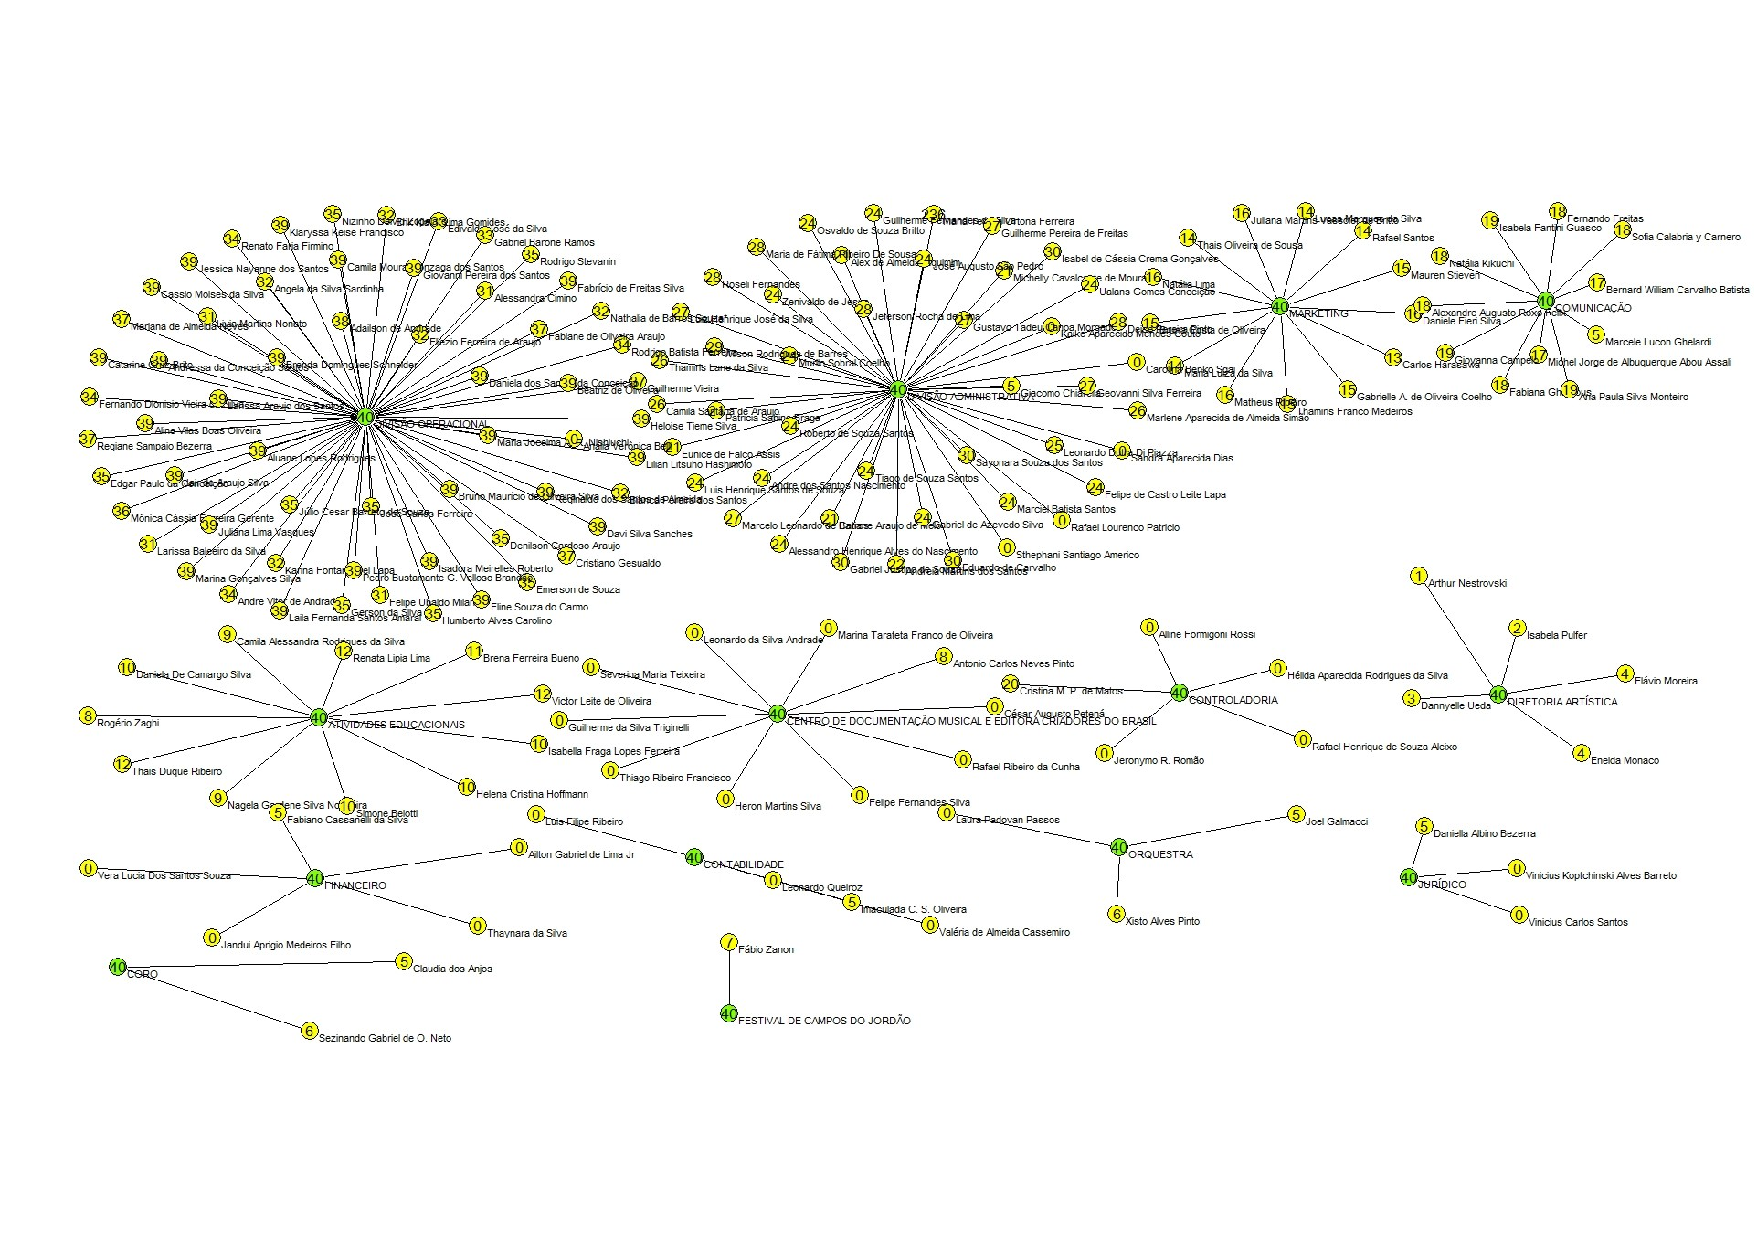
\includegraphics[scale=0.8]{OSESP_setores_pajek.pdf}

\fonte{Site da \citeonline{osesp2016site}. Dados trabalhados pelo autor.}

\end{sidewaysfigure}



\subsection{Financiamento}



Os recursos da OSESP provém de fontes diversificadas mas, sobretudo, diretamente do estado de São Paulo conforme o contrato de gestão vigente e, por outro lado, através da iniciativa privada. O Estado de São Paulo investiu, de 2010 a 2015 o montante de R\$251.676.666,67 distribuídos da seguinte forma: R\$7.166.666,67 em 2010, R\$43.400.000,00 em 2011, R\$53.400.000,00 em 2012, R\$55.500.000,00 em 2013, R\$55.650.000,00 em 2014 e R\$36.560.000,00 em 2015\footnote{O volume financeiro previsto para financiamento em 2015 a princípio era de R\$46.816.667,00 o qual foi alterado conforme o 6º termo de aditamento.}.



Em 2014 (dados mais recentes publicados), a OSESP teve um custo total aproximado de R\$100.327.000,00 e uma receita total aproximada de R\$102.339.000,00. A distribuição das receitas por suas fontes estão apresentadas na tabela TAL.



\begin{table}[ht]

\IBGEtab{

\centering

\caption{Distribuição das porcentagens de financiamento da OSESP}

}

{\begin{tabular}{rrr}

\hline

& Fonte & (\%)\\

\hline

1 & Projetos Incentivados & 35 \\

2 & Locação -- Eventos e Espaços & 18 \\

3 & Assinatura e Bilheteria & 18 \\

4 & Receitas Financeiras & 15 \\

5 & Permutas e Patrocínios & 11 \\

6 & Venda de Concertos & 3 \\

7 & Outras Receitas Próprias & 0 \\

\hline

\end{tabular}

}

{\fonte{Elaboração do autor a partir de \citeonline{osesp2014compromisso}.}}

\end{table}



Em 2014 a OSESP captou R\$18.190.000,00 junto à iniciativa privada (mediante isenção fiscal) e R\$15.548.000,00 em mídia por meio de permutas. As empresas financiadoras da OSESP estão divididas em 3 categorias conforme o volume de recursos investidos: patrocinadores (valores acima de R\$500.000,00), apoiadores (valores acima de R\%200.000,00)  e outros apoiadores (cf. Figura TAL). O Programa Sua Orquestra, programa de financiamento voltado à captação de recursos junto à pessoas físicas, reuniu 654 associados e arrecadou um montante de R\$980.000,00.



\begin{figure}[!ht]

\centering

\caption{Os investidores da OSESP em 2014}

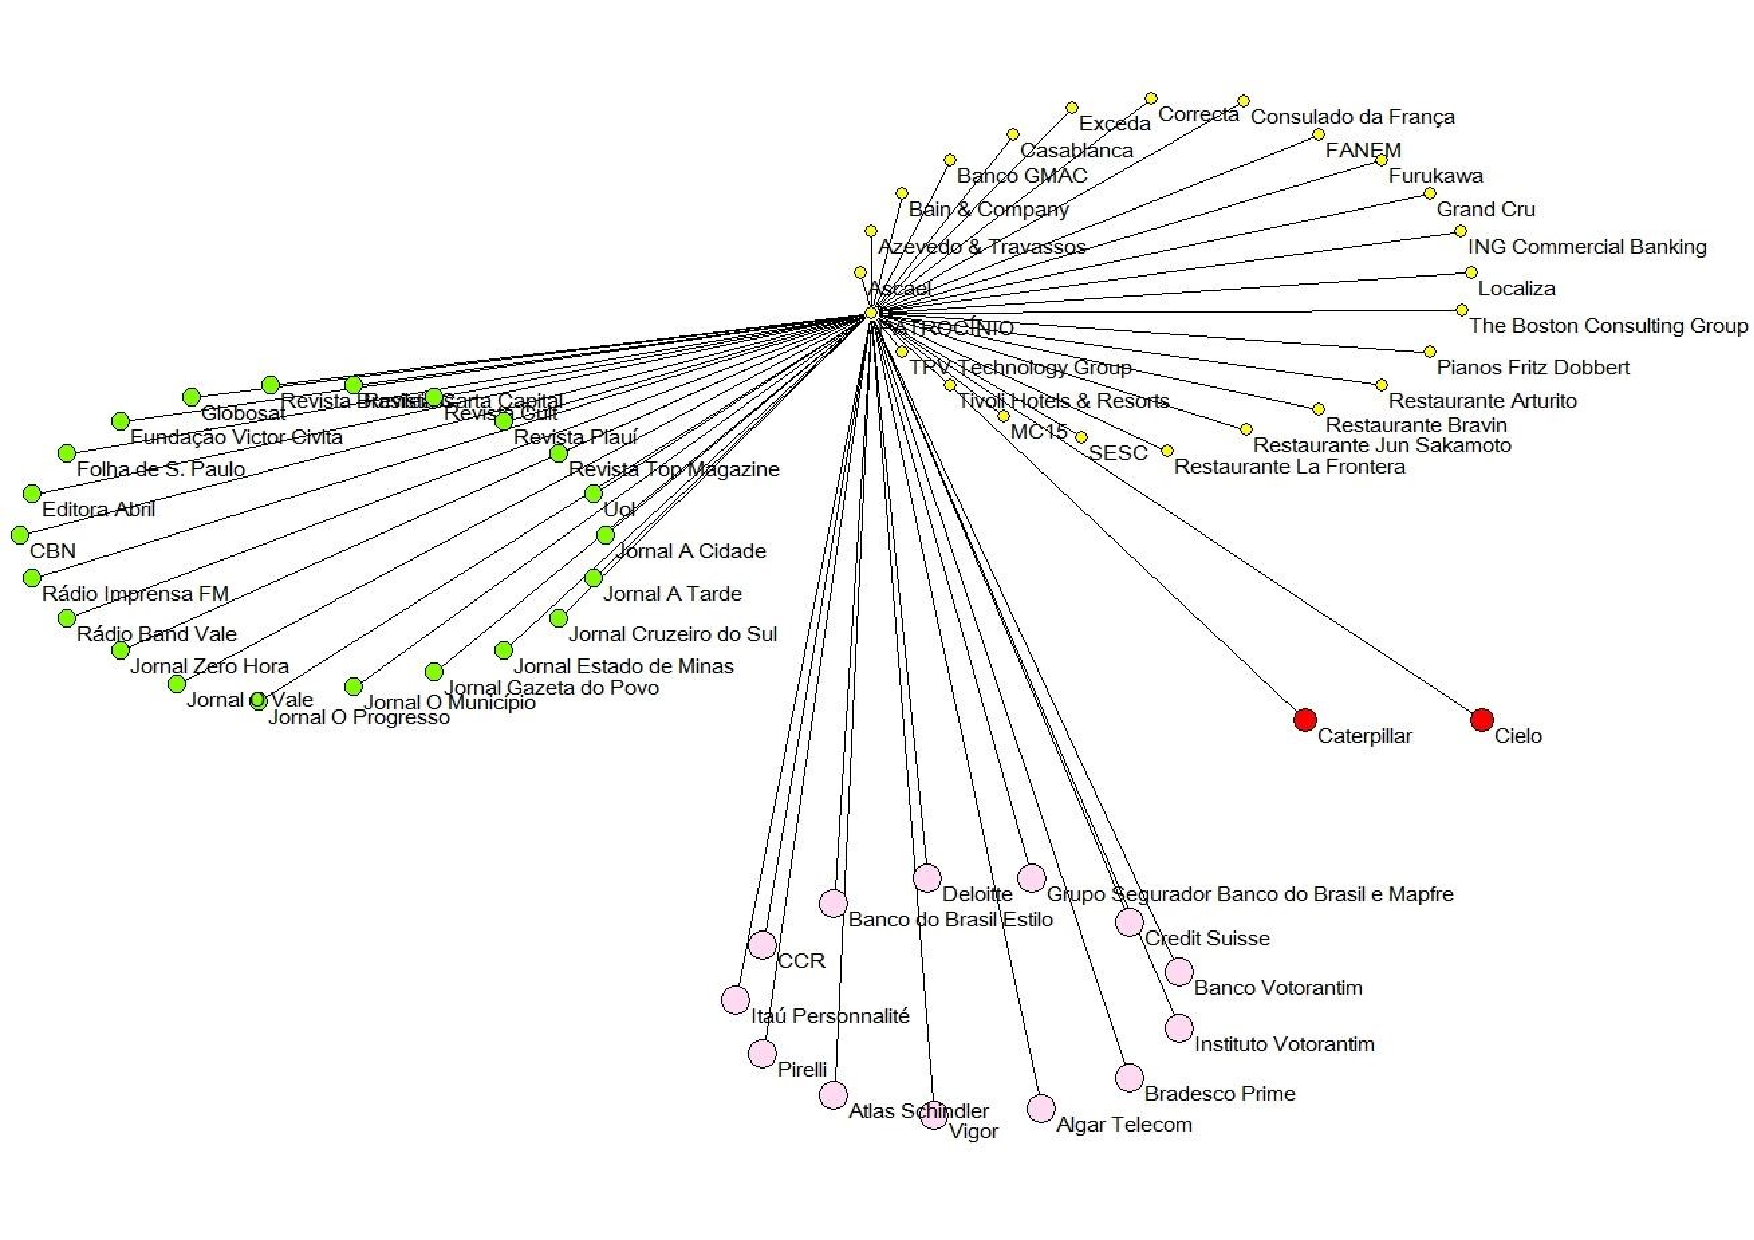
\includegraphics[scale=0.55]{OSESP_patrocinio.pdf}

\fonte{Elaboração do autor a partir de \citeonline{osesp2014compromisso}.}

\nota{Vértices rosas são patrocinadores, vermelhos são apoiadores, amarelos são outros apoiadores e verdes são veículos de comunicação parceiros via permuta. Com a exceção do grupo verde, o tamanho dos vértices indica as categorias de volume de investimento.}

\end{figure}









% Parei aqui!!!!!!!!!!

%=================================================================

%=================================================================

\end{comment}
